\chapter{Methodology} \label{chap:Methodology}

There are many unpredicted aspects that can result in unwanted images in real world screen environment.
For this reason, many algorithms were reviewed in the previous section to give an idea of the project scope.
Preprocessing step is a must to have better results, get a noise free image and to be able to specify the disease location clearly, then to develop an algorithm to track or classify it.
For some drawbacks in the algorithms reviewed regarding accuracy, speed and sensitivity and etc, we have introduced an automatic algorithm to classify the OCT volumes based on the Data provided SERI and OPTIMA.
Another algorithm is introduced in the project, which is classifying potential regions in the OCT images using the auto-encoder.
In this chapter, we present the method for both algorithms.
A MATLAB code implementation is developed using the cluster provided by University of Burgundy with Xeon 2630 V3 processor, 128 GB of RAM and a GPU Nvidia Tesla K40 which processes the algorithms proposed in an average of 5 hours per tasks.

\section{Introduction}

Many systems for retinopathy automatic detection in OCT images have been improved.
The results obtained is promising and discussed in the next chapter.
The machine used to train this system proposed is powerful to process a very big data in some hours where normal computers might take days to weeks to achieve the same task.
Algorithm used to correct the images light or contract increasing is used in the pre-processing section.
However, the image enhanced has limited resolution obtained cause sometimes increasing the threshold will yield to over-blurring , which is not good due to info losing might be useful.
Feature extraction in the images is also taking time to process meanwhile the multi-pyramid way is used.
In addition to those, feature representation is used to have a clear dictionary to the classifier.

Accuracy quality of results validation is a subjective concept to be determined.
It is not a straight task to be determined and this can be noticed with the different experts opinions  in term of making a decision of the same aspect.
To detect a disease that attacks the eye, same imaging technique is useless.
The reason behind that, in Glaucoma we need dark images to better figure out the nerves problem, while dark images are considered low quality if we want to detect Diabetic Retinopathy(DR).
Hence, we used confusion Matrix based on how many volumes detected as Normal, DME or wrong for both cases for the first part of the Project.

The second part, is using deep learning technique to train the data after extracting the potential regions using the MSER.
The classification is performed by assigning a label to the cyst location then fitting it to the auto-encoder.
Then we have a test data with their ground truths to be sent for prediction based on the cluster or network created from the auto-encoder.
Accuracy decision is made based on confusion matrix and compared with the two ground truth provided by OPTIMA laboratory and the intersection between them.  

Processing speed is another aspect to be taken into account when processing the algorithms, hence a powerful computer is in need for training and classifying the data about.
This chapter explains the methodology of the algorithms and it is divided into two parts, first is OCT classification based on machine learning techniques and the second is the OCT classification based on deep learning techniques. 

\section{Automatic classification Of OCT Volumes}

Inspired by the previous methods and using machine learning tools to obtain an automatic machine able to make a decision.
A supervised learning algorithm is designed to map a certain function with a known inputs and outputs.  
Our classification pipeline is depicted in Fig.3.1.
The rest of the section present into details each intermediate step.
Our approach is based on the original paper of Srinivasan et al\cite{srinivasan2014fully}.
It has been enhanced with feature representation like PCA , proposed in  \cite{venhuizen2015automated} and BoW.
Different classifiers are used and the results presented in the next chapter

\begin{figure}[htb]
        \centering
        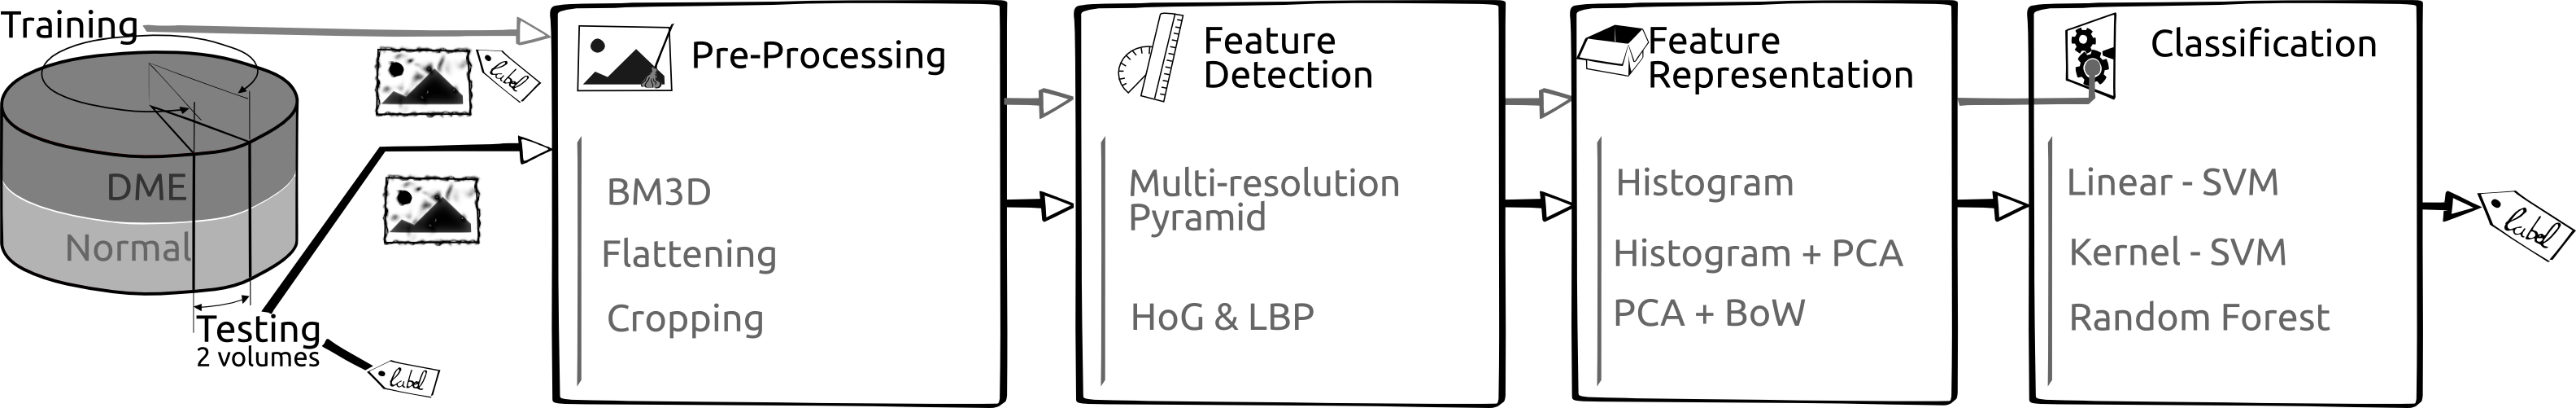
\includegraphics[width = 1\textwidth]{figures/Khaled-ICPR-method.png} % scale, width, height 
  \caption{Classification Pipeline}
  \label{fig:Classification Pipeline}
\end{figure} 

\subsection{Preprocessing}

Image blurring and sharpening is essential and critical step in machine learning aspects to ensure the high quality of the data presented to by analysed in a process called preprocessing.
Fixing the imperfections in the images is important to let the following tools useful.
So, this process is the main basis of images processing field. 
This project introduces the first step as Preprocessing as shown in the figure 3.2 the original image.
A sample of the image is shown here:
\begin{figure}[htb]
        \centering
        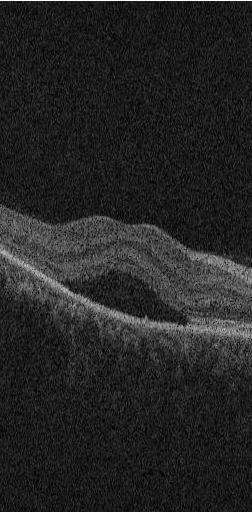
\includegraphics[width = 0.3\textwidth, height = 0.2\textheight]{figures/Original-image.jpg} % scale, width, height 
  \caption{Original B-scan slice}
  \label{fig:Original image}
\end{figure}

Following the work done by Srinivasan et al. \cite{srinivasan2014fully},and prior to feature extraction, the OCT volumes are pre- processed through de-noising, flattening, and cropping steps, the details as follow:
\begin{enumerate}
\item \textbf{De-noising}:It is the process of affecting the look of a certain image, by modifying pixels and its neighbours by some math equations applied to the images matrices.
Applying some filters to a particular images to enhance the look and remove the noise away.
In this part of the project we have used Block Matching 3D filtering to sharpen the image as shown in figure 3.3.
In the first step, speckle noise is attenuated through an image de-noising strategy which uses block matching and collaborative filtering in the 3D domain \cite{dabov2007image}, namely Block Matching 3D filtering (BM3D).
The core algorithm is composed of three steps: 
\begin{itemize}
\item \textbf{grouping}: consists in grouping similar 2D image patches from different spatial locations, to form 3D blocks.
\item \textbf{collaborative filtering} : is equivalent to de-noise the 3D blocks by successively applying a 3D transform, a de-noising method, and an inverse 3D transform.
\item \textbf{5 aggregation}:a de-noised 10 image is reconstructed by making a linear combination of the 2D de-noised patches. The previous algorithm is applied twice in the BM3D frame- work to build:
\begin{enumerate}
\item \textbf{basic estimate}: is computed by grouping 15 noisy 2D patches, de-noising the blocks via hard-thresholding with the value of 190, and aggregating the patches by setting the weights to be inversely proportional to the total sample variance of the blocks.
\item \textbf{final estimate}: the grouping is built from two distinct blocks by arranging 2D patches from both the
20 noisy image and basic estimate.
\end{enumerate}  
\end{itemize} 
The filtering is performed through a Wiener filter driven by the blocks extracted from the basic estimate, considered as the true energy spectrum.
The aggregation step is equivalent to the one performed in the basic estimate stage to obtain the final denoised image.

\begin{figure}[htb]
        \centering
        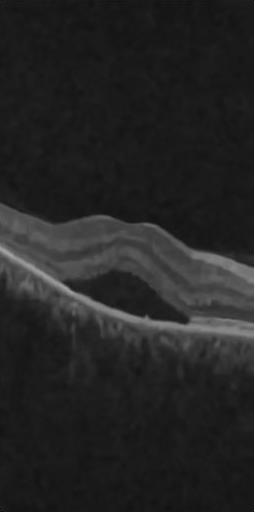
\includegraphics[width = 0.3\textwidth, height = 0.2\textheight]{figures/Denoising.jpg} % scale, width, height 
  \caption{De-noising B-scan Slice}
  \label{fig:Denoising image}
\end{figure}
\item \textbf{Flattening}: is the function used to make the layers of an image almost straight based on the function applied either fitting a polynomial or RANSAC.
SD-OCT images of the retina have a natural curvature as noticed in the figure 3.2, which is further distorted due to the common practices in OCT image acquisition and display that varies both between patients and within each SD-OCT volume.
Following Srinivasan et al. way we reduce the effects of the perceived retinal curvature when classifying SD-OCT images, we flatten the retinal curvature in each image.
To flatten the retinal curvature in each SD-OCT image:
\begin{itemize}
\item calculate a pilot estimate of the retinal pigment epithelium layer (RPE).
\item calculate the convex hull around the pilot RPE points, and use the lower border of the convex hull as an estimate of the lower boundary of the retina.
\item remove outliers by applying a [1 * 3] median filter (MATLAB notation) to this estimate.
\item Unlike Srinivasan et al. in his work for creating the flattened image, he fitted the second order polynomial to make the estimation of retinal lower boundary points.
Random Sample Consensus(RANSAC) function is applied to do the same job with better accuracy of line allignment.
An iterative method to achieve parameter estimation of a model from set of data with outliers.
With the accuracy achieved in RANSAC but there's a disadvantage of time as it has no limited time to do the job, until it finds the best alignment it will stop, otherwise it will continue calculating.
\end{itemize}
\begin{figure}[htb]
        \centering
        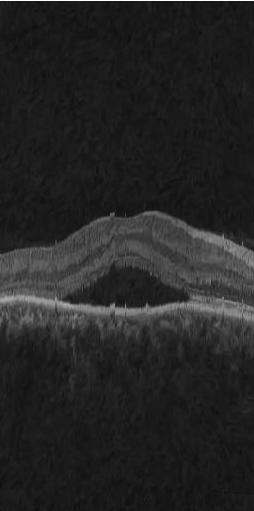
\includegraphics[width = 0.3\textwidth, height = 0.2\textheight]{figures/flattening.jpg} % scale, width, height 
  \caption{Flattening B-scan Slice}
  \label{fig:Flattening image}
\end{figure}

\item \textbf{Cropping}:this method is used to crop the region interested to save time when the data required for classification might take time.
Thus, to differentiate between the volumes with disease or not, limiting the targeted place might help the classifier to set the data clearly.
The cropping in our SERI data is bigger than the cropping region done by Srinivasan et al.
In the axial dimension, all images are cropped 325 pixels from over the RPE and 30 pixels under the RPE.
In the lateral dimension, all images are cropped 340 pixels to the center.
\begin{figure}[htb]
        \centering
        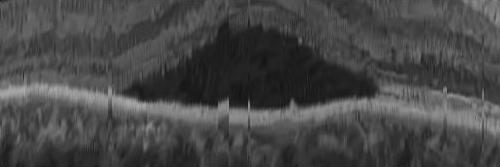
\includegraphics[width = 0.3\textwidth, height = 0.2\textheight]{figures/cropping.jpg} % scale, width, height 
  \caption{Cropping B-scan Slice}
  \label{fig:Cropping image}
\end{figure}

\end{enumerate} 

\subsection{Feature Extraction}

This part of the pipeline is meant to create informative data from measured data and build values (features), which they are non-redundant and lead to better interpretations.
It is crazy to take all features and in our case it reached up to 113215 dimension for 32 volumes, which real data is lost, only 32 points in this great number of dimensions.
It describes content of the features in images, algorithms and application and so on, 
This process finds out the connection between pixels in a particular image.
Descriptors describe the main characteristics such as shape, texture and many other aspects in image.
Descriptors are  divided into two groups:
\begin{itemize}
\item \textbf{General information descriptors}: give description of colour, shape , texture, basically low level descriptors.
\item \textbf{Specific domain information descriptors}: give description about events or objects like face recognition.
\end{itemize}

In the pipeline, implementation of Histogram of Oriented Gradients (HOG) and Local binary patterns (LBP) is applied and the explanation as follow:
\begin{enumerate}
\item \textbf{Histogram of Oriented Gradients (HOG)}: is a feature descriptor for object detection.
This descriptors are used based on gradient orientation in well-localized portion in an image.
It is computed based on overlapping local contrast normalization on a dense grid on uniform cells to enhance the accuracy.
HOG descriptors divides the image into connected cells by counting the the strength and orientation of the gradient spatial in every cell and computing the gradients can be done by applying the 1-D centred, point discrete derivative mask in one or both of the horizontal and vertical directions.
Applying the mask for filtering the color or intensity data of the image with some filter kernels like:[-1, 0, 1] or its transpose.
After that, HOG creates cells histograms in each pixel within the cell.
Each pixel has a weight for vote in an orientation-based histogram channel based on the values found in the gradient computation.
The cells shape can be radial or rectangular, and the histogram channels are evenly spread over 0 to 180 degrees or 0 to 360 degrees, relying on whether the gradient is unsigned or signed. 
To make the descriptors invariant to shadowing and different illumination, descriptor vectors blocks are normalized over larger overlapping blocks then renormalizing.
This results into a feature vector for each image with normalized histograms.
This technique is focusing more into edges unlike LBP which focuses in intensity of regions.

In our implementation, as Srinivasan et al. did, the extraction of HOG with [4*4] cell size, [2*2] cells per cell, a block overlap of [1*1] cells, unsigned gradients and 9 orientation histogram bins.
Extraction of HOG features at four levels of the multi-scale Gaussian low-pass pyramid to have multiple scale levels structure.
Furthermore, concatenate all HOG vectors for each image to obtain the set of histograms to be ready for the feature representation or classification.  
\item \textbf{Local binary patterns (LBP)}: is a visual descriptor and usually combined with HOG to improve the performance of detection on some dataset as our implementation did.
It starts with dividing the window of an image to cells (8*8 pixels for every cell).
After that, a comparison of each pixel with its 8, 16 and 24 neighbours with different radius of 1,2 and 3 based on the number of neighbours.
Followed by clockwise or counter-clockwise circle along the pixels.
The decision making in this process, "0" value is assigned to the pixel if the center pixel value is greater than neighbour’s value, otherwise assign value "1".
Then, the histogram is computed over the cell by the appearing pixels frequency based on the threshold of higher or less than the center.
In this project, Non-invariant rotation LBP and invariant rotation LBP are used.
Rotation Non-invariant (NRI)LBP is the same as the normal LBP where it results into a histogram of 255 size and this NRI LBP is not grouping the equal patterns into one histogram but it will just add it.
Unlike rotation invariant (RI)LBP that will group the equal patterns and put them into single histogram and this will reduce the histograms numbers for example from 255 to 50. 
Normalizing the vector feature is done.
Finally, concatenating all histograms from all cells in all images to make $128$ vectors for all volume.
this data is ready to be directed for further feature representation or directly to the classifier.
\end{enumerate} 

\subsection{Feature Representation}
The great number of dimensions resulted from the previous section make the processing time high for classification, hence classification loses the main points in the huge dimensions.
Many correlated feature vectors are produced, which reduces the precision and performance of system, so it is very crucial to learn the most important and uncorrelated features.
In another words, Feature representation is the way to create a new space for features either by making a new model for features or reducing the real features to more meaningful dimensions. 

There many types of feature representation methods, like Linear Discriminant Analysis (LDA), Principal Component Analysis (PCA), Sequential Forward Feature Selection (SFFS) and Sequential Backward Feature Selection (SBFS).
SFFS and SBFS are used to chose the most correlated dimensions, while PCA and LDA are projecting data into new space by reducing dimensions.
Bag of Words (BoW) is a feature representation method that try to find similar patterns based on creating dictionary or words in clusters for features in the space.
This section will explain the methods we used in the pipeline:
\begin{enumerate}
\item \textbf{Principal Component Analysis (PCA)}: is feature reduction method for the extracted data, which looks for subspaces where variation is maximized.
It is unsupervised, statistical orthogonal linear transformation approach where the subspace transformed data is relevant and uncorrelated .
The process of PCA basically, is done by picking up the highest variance value in the dimension till it reaches to the number chosen to be reduced.
The principal components are orthogonal transformation because they are the eigenvectors of the covariance matrix, which is symmetric.
PCA is sensitive to the repetitive scaling of the original variables, hence reducing the dimensions can not be achieved, a kernel of PCA is used to find subspaces.

PCA is the way of fitting some data from a lot of dimensions where each axis means a principle component.
Sometimes if the axis is small compare to others so the variance along the axis is small, hence the lose of some useful information is happened by deleting that axis. 
The math way of PCA is organized as follows
\begin{itemize}
\item subtracting the mean from each point in the dataset to gather data around origin center.
\item Calculating the covariance matrix of centred data.
\item Computing the eigenvectors covariance matrix corresponding eigenvectors.
\item Orthogonalizing eigenvectors sets then converting them to unit vectors by normalizing the eigenvectors.
\end{itemize}

In this project, reduction of HOG and LBP dimensions to 40 and 20 dimensions respectively.
The dimensions reduced are concatenated before BoW applied for creating dictionary of the data.
Mainly, the reduction was done based on Singular value decomposition (SVD), due to the accuracy produced with acceptable processing speed.
The avoidance of using Eigenvalue decomposition (EIG) cause the less accurate results generated compared to SVD, even-though it is faster.
There is another method to reduce feature data in PCA using Alternating least squares (ALS) algorithm, which can work well for data sets with a small percentage of missing data at random, but might not perform well on sparse data sets\cite{jackson2005user}.

\item \textbf{Bag of Words (BoW)}: is a clustering method for the extracted data by modelling them to a new space.
The number of repeating of pattern will make the decision how to cluster the data.
Clustering belongs to the use of k-means to make the cluster for the feature space so that k represent the number of words, histograms or samples number of minority class.
Hence, the centroids of these clusters define the new samples from the majority class.
BoW clusters are the set of low-level features using a k-means algorithm to produce a “codebook” of “visual words”.
Every visual word have a centroid that belongs to a cluster.
After generating the words, every centroid is represented by histogram based on the number of the occurrence of the words from extracted features \cite{sun2012automatic}.
K-means algorithm is an iterative method, which finds k centroids by alternating assignment and update steps.
Euclidean distance method is used for alternating assignment.
In this project, many tests involved using different number of k centroid and vary between 10-60.
The results of BoW will be shown in the next chapter.
\end{enumerate}

\subsection{Classification}
Classification is a method used to map an input data to its category.
This terminology task is to recognize the pattern after giving some data similar to it in a process called training.
Training might be attached with labels to be supervised learning or without labels to be unsupervised learning.
This part of the project is using supervised learning method with labels for Normal volumes and another label for DME volumes.
Three different classifier are used for comparison: Random Forest (RF), linear, and kernel- Support Vector Machine (SVM).
Using the feature descriptor provided the first two representations.
The classifiers are trained to classify B-scans and volume classification is performed based on the total number of diseased B-scans per volume using a majority vote rule and cross validation.
Here in this section we explain briefly about the classifiers used as follow:
\begin{enumerate}
\item \textbf{linear-Support Vector Machine (SVM)}: is a supervised learning algorithm based on training feature vectors to categorize whatever number of categories.
SVM creates set of points in space for a category then divided by a reasonable gap and make line to separate points for each category\cite{vermeer2011automated}.
The new separation of points mapped and predicted to make a decision for the classifier as shown in the SVM figure.
In this part, we used the Matlab function svmtrain but it did not converge then we used fitcsvm function with predict function to classify data.

\begin{figure}[htb]
        \centering
        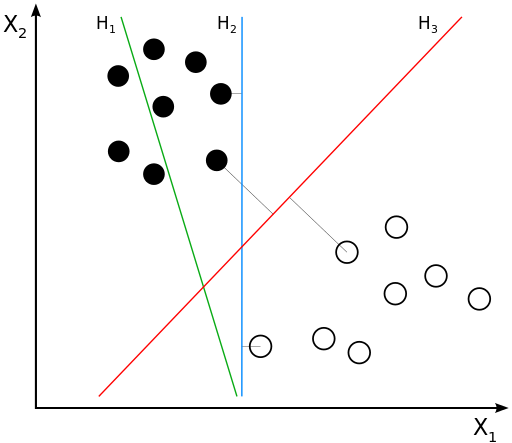
\includegraphics[width = 0.45\textwidth]{figures/SVM.png} % scale, width, height 
  \caption{Linear-SVM \cite{SVMmethod}}
  \label{fig:SVM}
\end{figure}

\item \textbf{kernel-Support Vector Machine (SVM)}: is exactly the same process of linear SVM but in non-linear way to maximize-margin hyperplanes, as shown in the figure 3.7.
This classifier is changing every dot product with the non-linear kernel function.
This allows to achieve the maximize-margin hyperplanes in the feature space transformation.
The plane might not by linear from input data to be transformed as shown.
Working in a higher-dimensional feature space will increase the chances of producing the generalization error of support vector machines, although given enough samples the kernel achieve good performance.
Here fitcsvm is the Matlab function used to perform this part with kernal RBF.
\begin{figure}[htb]
        \centering
        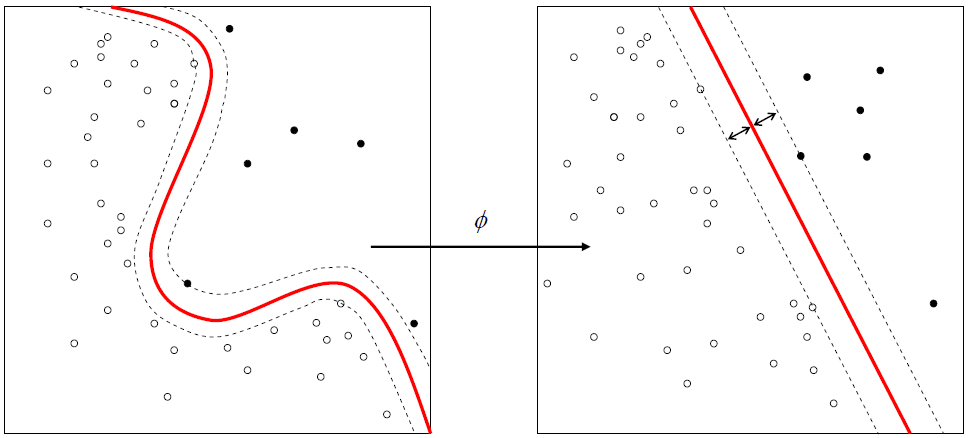
\includegraphics[width = 0.45\textwidth]{figures/Kernel_Machine.png} % scale, width, height 
  \caption{Kernal-SVM \cite{SVMmethodkernal}}
  \label{fig:SVM}
\end{figure}

\item \textbf{Random Forest (RF)}: is a classifier that creates trees and then sub-tress based on the targeted number of trees wanted to be involved in the classification task.
The more trees to create in this random forest the more time required to compute and the more details that process obtained.
This classifier is averaging many trees and sub-trees decision.
The average taken is trained on different features in the training set to reduce the variance.
This method uses the modified bagging algorithm, which selects random sample with replacement and fits trees into the samples, which differs from the bagging algorithm that targets to decrease the variance which will lead to better performance without even increasing the bias.
This means, increasing the number of trees will yield to correlated trees and this will increase the sensitivity to noise, hence bootstrap sampling will de-correlate the trees.

This classifier is enhancing the performance usually, but sometimes with the increasing of trees number the results might stay the same so in here \cite{oshiro2012many} proved that between 64-128 trees are performing good in term of accuracy, memory and time required.
In our project we aimed for 80 trees and results shown in next chapter. 
\end{enumerate} 
\subsection{Evaluation Of Classification}
This section briefly explains the way used to validate and evaluate the results obtained from the classifiers mentioned in the previous section.
The results were having the assessment based on:
\begin{itemize}
\item \textbf{Validation}: is the way to generalize the classification results.
In this section, we performed leave-two-patient-out-cross-validation, where we take the first voxel from DME images and first voxel from normal images out for testing and the 30 other volumes are processed for training.
After that, changing the testing set by substituting the first voxel with second voxel and so on ... 
for 16 times because we have 32 volumes.   
\item \textbf{Evaluation}: is a method to make results shown and determines the method quality for further comparison.
A confusion matrix is done to classify the results and in our case the confusion matrix has two rows and columns, because we classified based on the volume type either diseased or normal.
\begin{figure}[htb]
        \centering
        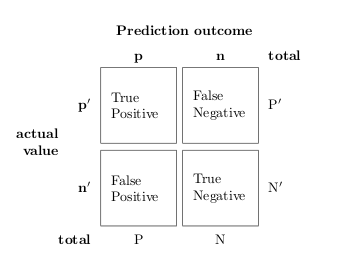
\includegraphics[width = 0.45\textwidth]{figures/Confusion.png} % scale, width, height 
  \caption{Confusion Matrix for evaluation \cite{confusion}}
  \label{fig:Confusion}
\end{figure}

The figure shows the evaluation way followed in this project as the True positive (TP) and true negative (TN) are the samples that are correctly predicted to belong to the disease or normal class, respectively.
False positive (FP) and false negative (FN) are predicted as the FP in the negative class while it is in the positive class and vice versa.
The confusion matrix is the famous method to compute the accuracy (ACC), sensitivity (SE), specificity (SP), and precision.
The equations to calculate the accuracy, sensitivity are shown in equation 3.1 and 3.2 respectively.
Another aspects used to evaluate the method performance like F-score and Precision.
\begin{equation}
Sensitivity = \frac{TP}{TP+FN}
\end{equation}
and,

\begin{equation}
Specificity = \frac{TN}{TN+FP}
\end{equation} 
and,

\begin{equation}
Precision = \frac{TP}{TP+FP}
\end{equation}
\end{itemize}

\section{Automatic Classification Of Potential Regions in OCT Volumes}
Inspired by deep learning techniques and the segmentation methods discussed in section 2.2.2, this algorithm is introduced to classify the potential regions inside an image.
This section is explaining the method used to classify the OPTIMA challenge data as shown in figure 3.9.
The rest of the section present into details each intermediate step.
This method is based on extracting Maximally stable extremal regions (MSER) ''threshold set empirically'' and then cropping each region.
After that, comparing the cropped images with the Simultaneous truth and performance level estimation (STAPLE) mask images is used for label validation.
The total patches extracted from training data and testing data are  354311 and 113149 patches ,respectively. 
Assigning the patches with labels are fit into auto-encoder for learning and feature extraction, then classification followed by comparing the testing data with the network built in the autoencoder to validate the results.

\begin{figure}[htb]
        \centering
        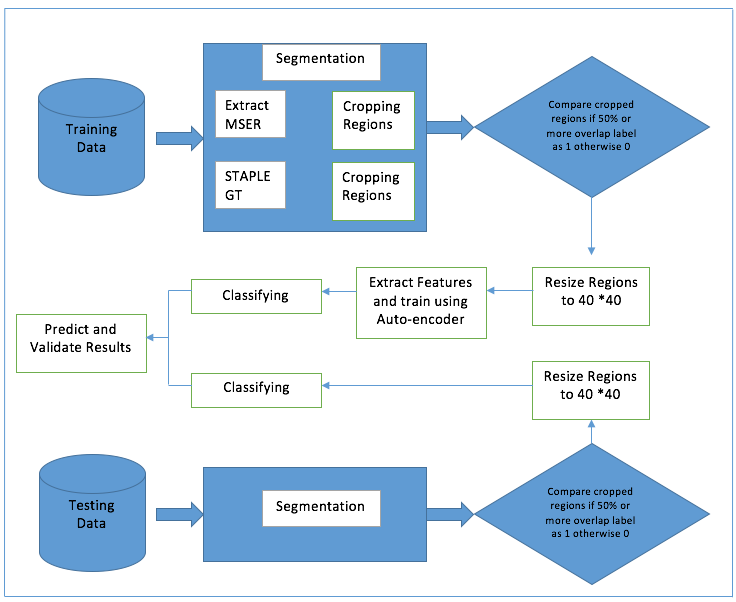
\includegraphics[width = 0.9\textwidth, height = 0.5\textheight]{figures/Segmentation.png} % scale, width, height 
  \caption{Cyst Classification Pipeline}
  \label{fig:Segmentation Pipeline}
\end{figure} 
\subsection{Segmentation Process}
This section explains the steps used to segment an image as many researchers proposed many methods as shown in chapter 2.2.2. and for this project we segment the potential regions as follows:
\begin{enumerate}
\item\textbf{Maximally stable extremal regions (MSER)}: is a method used as blob detection in images.
This algorithm proposed by Matas \cite{matas2004robust}, is extracting regions based on the differ of intensity between image elements and create stable regions or images inside each image.
This method led to better matching of certain regions with a very fast speed of extracting each image and to compare it with other regions in other images and has the following steps to extract regions:
\begin{itemize}
\item Sorting pixels by intensity.
\item Marking the set of pixels of each region in different color and the list of merging connected components using union-find algorithm.
\item Data structure is produced as a function of intensity of connected pixels.
\item two components are merged into larger region if the two groups are smaller than the threshold value set to form one region.
\item Regions presented are the the results of the stable regions over large range of threshold.
\end{itemize}
We extracted MSER regions, which has the cyst regions and non-cyst regions in all images of the training and testing data.
\begin{figure}[htb]
        \centering
        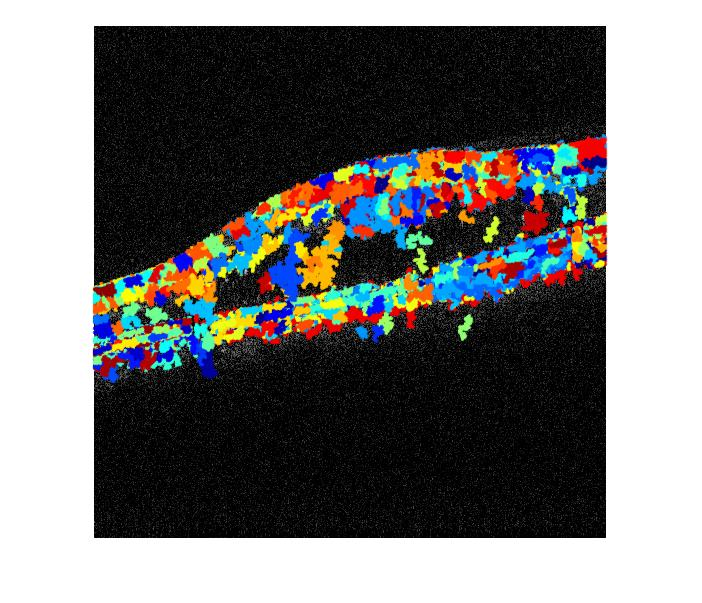
\includegraphics[width = 0.6\textwidth, height = 0.4\textheight]{figures/MSER.jpg} % scale, width, height 
  \caption{Maximally stable extremal regions}
  \label{fig:Segmentation Pipeline}
\end{figure} 
\item\textbf{Simultaneous truth and performance level estimation (STAPLE)}: is a method used for the validation of segmenting image.
The challenge of having optimal method to segment an image is still under research due to the differences in images and resolution.
Evaluating the performance of certain algorithm in image segmentation is a difficult process.
The reason behind that is back to different opinions of raters or experts in deciding how to make ground-truth suiting an image condition, hence the existence of STAPLE to form one ground-truth of all ground-truth presented for one image.

STAPLE is removing the variability introduced by raters to ensure the quality of the proposed method to segment.
This method is considering a collection of pixels representing the segmentation and then computing the probabilistic estimate of the true segmentation.
The probabilistic estimate of the true segmentation is achieved by predicting the optimal combination of the raters segmentation, weighting each segmentation based on the estimated performance level.
Then, incorporating a prior model for the spatial distribution of structures being segmented, as well as spatial homogeneity constraints.
STAPLE is a straight method to use and apply in clinical imaging data, it can enable assessment of the performance of an automated image segmentation algorithm, and enables direct comparison of human rater and algorithm performance\cite{warfield2004simultaneous}.
OPTIMA data includes two ground truths and using STAPLE algorithm to generate a single ground truth, which contains the data of both ground truths for having a single reference instead of two.
\begin{figure}[htb]
        \centering
        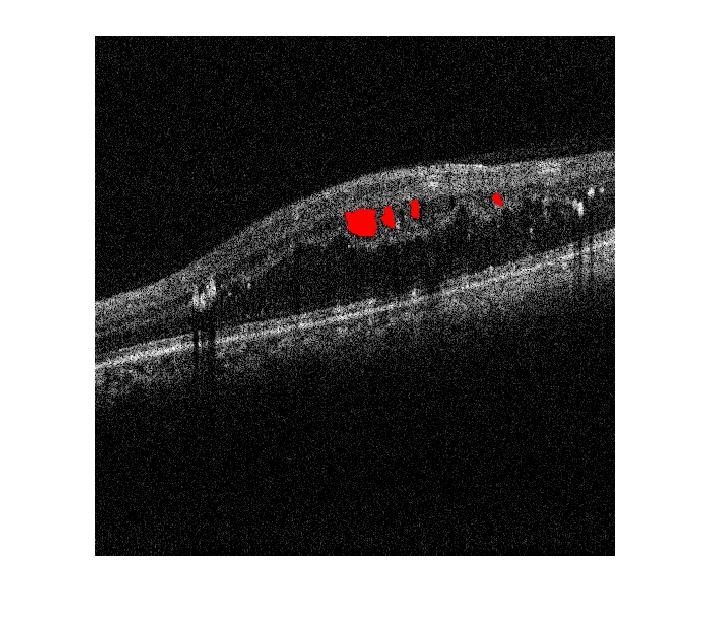
\includegraphics[width = 0.6\textwidth, height = 0.4\textheight]{figures/STAPLE.jpg} % scale, width, height 
  \caption{Simultaneous truth and performance level estimation}
  \label{fig:Segmentation Pipeline}
\end{figure}
\item\textbf{Labelling Patches}:is a process to compare regions extracted from MSER with regions extracted from STAPLE ground truth to assign a label for each patch and then resizing the regions to fit it to the auto-encoder.
\end{enumerate}

\subsection{Auto-encoder Training And Feature Extraction}
Auto-encoder is neural network which is copying the inputs to its outputs in the training process.
It has different hidden layers internally that represent the input data.
The network has two parts which are an-encoder function $h=f(x)$ and decoder which generate the reconstruction $r=g(h)$.
Usually auto-encoders are restricted in ways that allow them to learn to copy only input that feeds the training data.
Because the model is forced to prioritize, which aspects of the input should be copied, it often learns useful properties of the data and the structure of auto-encoder as shown in figure 3.12.
Typically, auto-encoders used for reducing the dimensions or feature extraction.

\begin{figure}[htb]
        \centering
        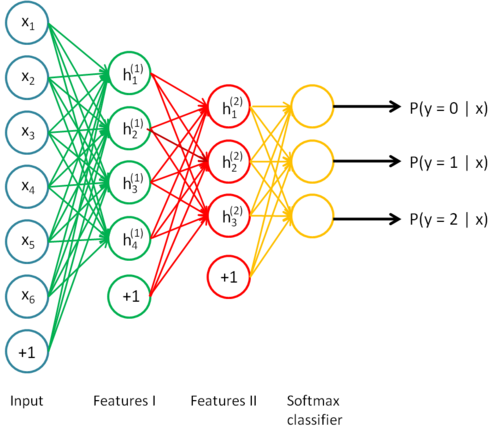
\includegraphics[width = 0.7\textwidth]{figures/Autoencoder.png} % scale, width, height 
  \caption{Autoencoder Layout}
  \label{fig:Autoencoder Layout}
\end{figure} 

Auto-encoder is used for training and the algorithm can be summed up as:
\begin{itemize}
\item Feed-forward each input $x$ to calculate the activations in all hidden layers and at the output layers to obtain $x'$.
\item Using squared error, measure the deviation of $x'$ from the input $x$.
\item Backpropagate the error and update the new weight in the net.  
\end{itemize}

Auto-encoder is trained using back-propagation (Fine tuning), which calculates the gradient of the loss function with respect to weights through the network.
The weights of this task can be shown in fig 3.13.

\begin{figure}[htb]
        \centering
        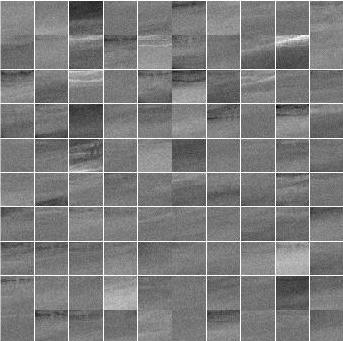
\includegraphics[width = 0.6\textwidth, height = 0.4\textheight]{figures/weightsautoencoder1.jpg} % scale, width, height 
  \caption{Weights of Auto-encoder}
  \label{fig:Segmentation Pipeline}
\end{figure}
This gradient is used to optimize the algorithm, which is used later to update the weights to minimize the loss function\cite{liou2014autoencoder}.
Backpropagation demands a known output for each input to compute the loss function gradient. 
This method is supervised and it is used in unsupervised method in auto-encoder.
Using backpropagation to train network with many hidden layers will make the first layer when it received the error insignificant, hence conjugate gradient method can solve this problem.
Another way to solve this slow process by setting initial weights that estimate the final output.
In this project, we train the autoencoder with 100 hidden layers at the first hidden layer then 50 hidden layers at the second layer. then it is classified using softmax layer classifier.

\subsection{Classification} 
The process of spotting the differences between various classes.
This process is explained in 3.2.4. 
In this part, SVM. or SVM-RBF or RF are not used, but Softmax layer is used instead for classifying the existence of the cyst or not.
Softmax layer is a generalization of the logistic function which is implemented at the last layer of the network.
\subsection{Evaluation And Validation}
This process is evaluated using the confusion Matrix.
Validation of the results was done based on the same aspects as in section 3.2.5 which they are Precision, Sensitivity and Accuracy.

 













